\documentclass[journal]{IEEEtran}
\usepackage[T1]{fontenc}
\usepackage[utf8]{inputenc}
\usepackage{cite}
\usepackage{amsmath,amssymb}
\usepackage{graphicx}
\usepackage{booktabs}
\usepackage{multirow}
\usepackage{array}
\usepackage{xcolor}
\usepackage{algorithm}
\usepackage[noend]{algpseudocode}
\usepackage{url}
\usepackage[hidelinks]{hyperref}
\graphicspath{{figures/}}
\newcommand{\placeholder}[1]{\textbf{\textcolor{red}{[#1]}}}

\begin{document}

\title{Single-Channel EEG Detection of N3 Sleep with Interpretable Slow-Wave Factor Scores: A Multi-Cohort Study with Multi-Scorer References}

\author{\placeholder{AUTHOR INPUT: author names, affiliations, institutional e-mail addresses, ORCID iDs; mark the corresponding author}%
}

\markboth{IEEE Journal of Biomedical and Health Informatics}{Single-Channel EEG Detection of N3 Sleep with Slow-Wave Factor Scores}

\maketitle

\begin{abstract}
\textit{Objective:} Automatic stagers label epochs only as deep (N3) sleep or not, although slow-wave strength varies within N3. We developed a single-channel electroencephalography method that detects N3 and describes detected epochs with transparent slow-wave measures. \textit{Methods:} A convolutional network with feature fusion and temporal context was trained on 251 recordings from two cohorts (participant-grouped cross-validation) and tested on five external cohorts. Detected epochs received rule-based factor scores, an additive rating, a grade and a reliability score. Success criteria were prespecified. \textit{Results:} The detector achieved a pooled cross-validated N3 F1 of 0.849; externally, F1 was 0.580--0.869 and the receiver operating characteristic area at least 0.96. In the hardest cohort, model-expert agreement was within the expert range. Trained identically, the detector matched DeepSleepNet, a model with 264 times more parameters, and outperformed three others in cross-validation. Factor scores decreased across the night, slow-wave morphology more steeply than the detector output (post hoc), and the rating rose with the fraction of experts scoring N3 (median within-participant correlation 0.81 across N2/N3 epochs, 0.56 within detected N3); the detector output followed votes more closely. The grade partly separated expert stage 4 from stage 3 (area under the curve 0.743, below the prespecified 0.75). Excluding the 20\% least reliable epochs raised F1 on the remaining epochs to 0.949. \textit{Conclusion:} One electroencephalography channel supports N3 detection with high ranking accuracy in all cohorts and an interpretable within-N3 description following slow-wave physiology. \textit{Significance:} Slow-wave sleep is linked to brain health; this open method measures it from one channel as a research tool, not a clinical score.
\end{abstract}
% abstract numbers: 251 (rq1_detection_metrics pooled n_participants), 0.849/0.838/0.861 (rq1_detection_metrics), 0.580/0.869 (external rows),
% 264 (ledger_extra DERIVED), 0.81 (research_question_results RQ2), 0.743 (rq2_rk_grade_validation), 0.949 (rq6_risk_coverage)

\begin{IEEEkeywords}
Electroencephalography, explainable artificial intelligence, external validation, slow-wave sleep, sleep staging, uncertainty.
\end{IEEEkeywords}

\section{Introduction}
\IEEEPARstart{D}{eep} slow-wave sleep (N3) is one of the most important states the brain enters each night. Its cortical slow oscillations are strongest early in the night and weaken as sleep pressure falls \cite{borbely2016twoprocess}, and the amplitude and slope of single slow waves decline with them \cite{riedner2007slowwaves,tononi2014plasticity}. In animals, sleep increases the removal of waste products such as $\beta$-amyloid from the brain \cite{xie2013clearance}. In community cohorts, less slow-wave sleep goes with more signs of brain ageing \cite{baril2021brainaging} and, over several years, with a higher dementia risk \cite{himali2023dementia}. Slow-wave measures are therefore promising markers for brain-health research, especially over many nights at home.

Three problems stand out. First, clinical scoring turns a graded process into one label: an epoch is N3 when at least 20\% of it has 0.5--2~Hz waves of at least 75~\textmu V peak-to-peak \cite{aasm2020manual}, whereas the older Rechtschaffen and Kales rules split this range into stage 3 (20--50\%) and stage 4 (more than 50\%) \cite{rechtschaffen1968manual}. An epoch that just passes the threshold and one full of large waves therefore get the same score. Second, the N2/N3 boundary is the least reliable decision in manual scoring: N3 agreement was only 67.4\% across more than 2,500 scorers in the AASM inter-scorer programme \cite{rosenberg2013interscorer}, and the fixed 75~\textmu V criterion is criticised because EEG amplitude varies with age and sex \cite{davidson2025n3,rosinvil2021age}. Third, N3 duration varies far more from night to night than slow-wave activity does \cite{qin2026swa,mullins2024stability}, so a count of N3 epochs is a rough summary of the physiology that matters most.

Single-channel EEG makes long-term recording practical, and deep learning stagers now reach expert-level agreement on such data \cite{supratak2017deepsleepnet,supratak2020tinysleepnet,eldele2021attnsleep,phan2023lseqsleepnet,perslev2021usleep,vallat2021yasa,phan2022review}. Their output, however, is still a binary label or a stage probability. Continuous depth measures such as the odds ratio product \cite{younes2015orp} and the sleep depth index \cite{zhou2025sdi} describe depth across all stages, not the strength of slow waves inside N3. What is missing is a single-channel method that finds N3, describes slow-wave strength in each epoch and night in clear physiological terms, and warns when its output should not be trusted.

This work presents such a method and tests it as strictly as public data allow. The detector learns from expert labels; the description uses fixed rules, because no dataset contains expert ratings of slow-wave strength and a model trained on its own input features would only confirm itself. We fixed seven research questions with two sub-questions and their success criteria before computing the full results, and report every verdict as computed. Across seven cohorts and 457 participants, the detector ranked N3 epochs almost as well in independent centres and devices as in cross-validation and matched or outperformed four published architectures retrained under the same protocol; the factor scores turned the binary label into a graded description that follows the night-time decline, age and the graded expert vote; and the reliability score flagged likely errors and, within ISRUC-I, the epochs on which the two experts disagreed.

The main contributions are:
\begin{enumerate}
\item A small single-channel N3 detector (96,226 parameters) with a dilated temporal-context block, evaluated with participant-grouped cross-validation on 251 participants and on five external cohorts, and compared with four published architectures retrained under the same protocol and with a pretrained open-source stager. % rq1_detection_metrics
\item Four rule-based factor scores (delta intensity, slow-wave morphology, spectral dominance and N3 continuity), an exactly additive overall rating, and a Low/Moderate/High slow-wave grade based on the published 20\% and 50\% coverage criteria.
\item An evaluation of the description against the homeostatic decline, the graded vote of two to five experts per epoch, expert Rechtschaffen and Kales stage 3 versus stage 4, age, and, descriptively, night-to-night stability.
\item A reliability score that keeps signal quality, confidence and out-of-distribution distance as separate inputs; removing the 20\% least reliable epochs raised F1 from 0.849 to 0.949 on the remaining epochs. % rq6_risk_coverage
\end{enumerate}

\section{Related work}
\subsection{Automatic N3 detection and single-channel staging}
Early slow-wave detectors relied on handcrafted spectral or time--frequency features and fixed thresholds; a recent one separates wake and N3 in one channel with Wigner--Ville features \cite{yeh2024n3}. Deep networks learn such features directly: DeepSleepNet combined convolution with recurrent layers \cite{supratak2017deepsleepnet}, TinySleepNet reduced its size \cite{supratak2020tinysleepnet}, and AttnSleep added temporal self-attention \cite{eldele2021attnsleep}. Sequence models showed that several minutes of context, or a whole sleep cycle, improves staging \cite{phan2022sleeptransformer,phan2023lseqsleepnet,phan2022review}. U-Sleep was trained on many clinical cohorts \cite{perslev2021usleep}, and YASA is open-source and trained on over 30,000 hours of recordings \cite{vallat2021yasa}. Published five-class N3 results differ in data, channels and splits, so we retrained four of these models on our own folds.

\subsection{Continuous descriptions of sleep}
Hypnodensities, which give per-stage probabilities, carry more information than hypnograms \cite{stephansen2018hypnodensity} and track disagreement among experts \cite{bakker2023ambiguity}; a supervised version mostly mirrors annotator behaviour, although its N3 output is linearly related to delta power \cite{huijben2023hypnodensity}. The odds ratio product \cite{younes2015orp} and the sleep depth index, learned from more than 10,000 recordings and linked to health outcomes \cite{zhou2025sdi}, describe depth across all stages. Slow-wave amplitude and slope mark homeostatic sleep pressure \cite{riedner2007slowwaves,tononi2014plasticity} and are usually measured with zero-crossing detectors \cite{massimini2004travelling}. To our knowledge, no automated single-channel method combines N3 detection with a decomposed, named description of slow-wave strength, tested against expert references and the homeostatic decline.

\subsection{Uncertainty and human disagreement}
The Dreem datasets provide five scorers per recording and a framework for comparing automated staging with their consensus \cite{guillot2020dod}. Soft-consensus labels improve training on such data \cite{fiorillo2023multiscored}, generative models reproduce inter-rater disagreement \cite{vangorp2023uflow}, and ensemble disagreement predicts scorer uncertainty \cite{dei2025sleepyland}. Entropy and Monte Carlo uncertainty have been used to send uncertain epochs to experts \cite{phan2022sleeptransformer,heremans2024upass} and work especially well for N2/N3 confusions \cite{vainikka2026uncertainty}, the boundary that human scorers also find hardest \cite{rosenberg2013interscorer}. We extend this to N3: our reliability score keeps its parts separate, and both the description and the reliability score are tested against graded expert disagreement.

\section{Materials and methods}
Fig.~\ref{fig:pipeline} and Algorithm~\ref{alg:pipeline} give an overview of the method. Only the N3 detector is learned; every score for detected epochs is a fixed rule applied to the signal.

\begin{figure*}[!t]
\centering
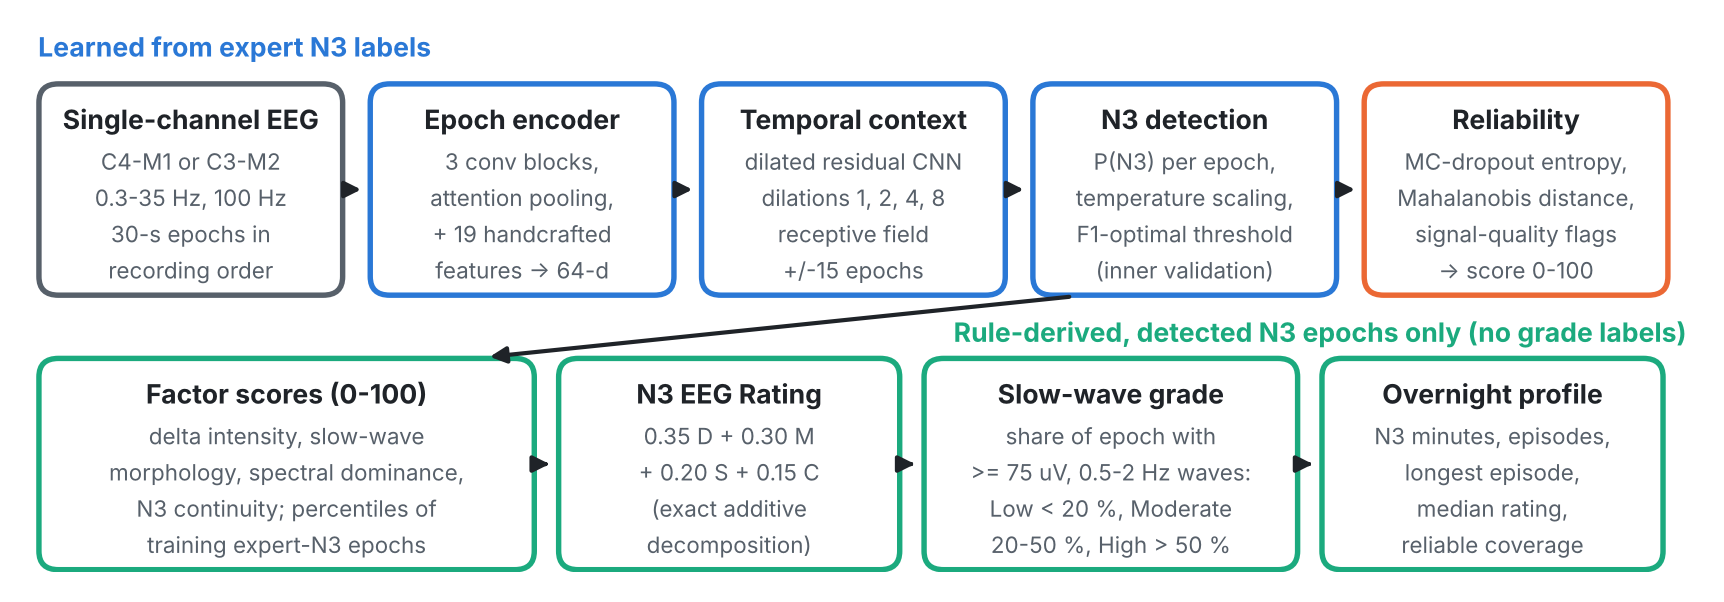
\includegraphics[width=0.62\textwidth]{fig_pipeline.png}
\caption{Overview. Top row: the detector is trained on expert N3 labels and gives a temperature-scaled N3 probability for each 30-s epoch; a separate reliability model combines model confidence, out-of-distribution distance and signal-quality flags. Bottom row: for epochs detected as N3, fixed rules calculate four factor scores and their additive rating and assign a three-level slow-wave grade; nightly summaries form an overnight profile. No grade or quality labels are used at any step.}
\label{fig:pipeline}
\end{figure*}

\subsection{Cohorts}
Table~\ref{tab:cohorts} lists the seven cohorts. ISRUC-Sleep subgroup I (100 adults recorded at a clinical sleep centre, two scorers) and the Haaglanden Medisch Centrum database (151 clinical recordings, one technician, AASM version 2.4) were the training cohorts \cite{khalighi2016isruc,alvarez2022hmcdb,alvarez2021hmc}. The other five cohorts were used only for testing: ISRUC-Sleep subgroup II (eight participants recorded twice, used for test--retest analysis), subgroup III (ten healthy participants) \cite{khalighi2016isruc}, the Dreem Open Datasets DOD-H (25 healthy volunteers) and DOD-O (55 patients with obstructive sleep apnea), each scored by five technicians from different centres \cite{guillot2020dod}, and the CAP Sleep Database (108 recordings scored with the Rechtschaffen and Kales rules, stage 3 and stage 4 separate) \cite{terzano2001cap,goldberger2000physionet}. CAP served only as the expert stage 3/4 reference for the slow-wave grade and for reporting detection; it is not part of the external criterion of the detection analysis. In total, the data contained 465 recordings, 437,430 epochs and 457 participants. % E: data_inventory.csv, run notebook cell 28 (465, 437430, 457)

For ISRUC, the reference label comes from the first scorer, and the second scorer is used only for inter-rater analyses. For DOD, the reference label is the majority vote of the five scorers; ties are broken by the scorer with the highest mean agreement \cite{guillot2020dod}. The public DOD-O signals are cropped at the start relative to the scorer hypnograms of the evaluation repository. We therefore matched the scorer consensus to the hypnogram stored in each DOD record, which is aligned with that record's signal, by choosing the epoch offset that maximised their agreement. This step uses labels only. All 80 records were matched (median offset 106 epochs in DOD-O; agreement at least 0.847); records with agreement below 0.6 would have been excluded. We found this misalignment after the first full run, and all reported results use the matched labels, with no change to the criteria or model settings. Because the matching depends on labels, its possible effect on the DOD results has not yet been checked with a label-free alignment (Section~\ref{sec:limitations}). % E: ledger_extra 80, 106, 0.847; methods_parameters.csv DOD reference

\begin{table}[!t]
\caption{Cohorts. Epochs are expert-scored 30-s epochs; N3 is the share of scored epochs in the evaluated set. Native rates were resampled to 100~Hz.}
\label{tab:cohorts}
\centering
\setlength{\tabcolsep}{3pt}
\footnotesize
\begin{tabular}{@{}llrrrrl@{}}
\toprule
Cohort & Role & Part. & Rec. & Epochs & N3 & Channel (native Hz) \\
\midrule
ISRUC-I & training & 100 & 100 & 90,187 & 0.194 & C4-M1 (200) \\ % data_inventory, rq1_detection_metrics cohort=ISRUC-I
HMC & training & 151 & 151 & 137,243 & 0.194 & C4-M1 (256) \\
ISRUC-II & external, retest & 8 & 16 & 14,207 & 0.184 & C4-M1 (200) \\
ISRUC-III & external & 10 & 10 & 8,889 & 0.229 & C4-A1 (200) \\
DOD-H & external, 5 scorers & 25 & 25 & 24,665 & 0.140 & C3-M2 (250) \\
DOD-O & external, 5 scorers & 55 & 55 & 53,236 & 0.105 & C4-M1 (250) \\
CAP & S3/S4 reference & 108 & 108 & 107,976 & 0.239$^{a}$ & C4-A1$^{b}$ (100--512) \\
\bottomrule
\end{tabular}
\vspace{2pt}

\raggedright\scriptsize HMC, Haaglanden Medisch Centrum; DOD, Dreem Open Datasets; Part., participants; Rec., recordings. A1 and M1 denote the same mastoid reference; ISRUC-I and ISRUC-II contain both labels. $^{a}$R\&K stage 3 + 4 share in the 105 evaluated recordings (three excluded, Section~\ref{sec:exclusions}). $^{b}$104 recordings C4-A1, four C3-A2. Age (mean $\pm$ SD) and sex from the source releases: HMC 53.9 $\pm$ 15.4 years, 85 men/66 women (151 recordings of release 1.1) \cite{alvarez2022hmcdb}; DOD-H 35.3 $\pm$ 7.5, 19/6; DOD-O 45.6 $\pm$ 16.5, 35/20 \cite{guillot2020dod}; CAP 44.8 $\pm$ 19.5, 62/40 (102 with age); ISRUC demographics were no longer retrievable.
\end{table}

\subsection{Signal processing}
\label{sec:exclusions}
From each recording we used one central derivation, C4-M1 (or C4-A1, which has the same mastoid reference), or otherwise C3-M2; no other channel was ever used instead. One ISRUC-I recording stored monopolar channels and was re-referenced as C4$-$A1. Signals were band-pass filtered at 0.3--35~Hz (fourth-order zero-phase Butterworth), resampled to 100~Hz and cut into 30-s epochs (3,000 samples) in recording order. All scored epochs were kept; quality-control flags (amplitude, z-score, high-frequency power, clipping) were stored but never used to remove epochs. Three CAP recordings contained values outside the range of the 16-bit floating-point cache. They were excluded from all evaluations by a model-independent rule (non-finite cached signal), which we identified during the first analysis run and applied in the same way to all models. % methods_parameters.csv; evaluation_exclusions.csv (CAP n13-n15)

For each epoch we computed nineteen handcrafted features from a Welch spectrum (4-s Hann windows, 50\% overlap): absolute and relative power in the slow-delta (0.5--2~Hz), delta (0.5--4~Hz), theta, alpha, sigma and beta bands, delta/theta, delta/alpha and delta/beta log-ratios, spectral entropy, and slow-wave measures from a zero-crossing full-wave detector \cite{massimini2004travelling} (0.3--4~Hz band-pass; negative half-wave 0.25--1.0~s; full wave 0.5--2.0~s): wave count per minute, the share of the epoch covered by waves of at least 75~\textmu V, and the median peak-to-peak amplitude and ascending slope of candidate waves. The features were standardised with the median and interquartile range of the training fold and clipped at $\pm$10 interquartile ranges.

\begin{algorithm}[!t]
\caption{Detection and description of one recording}
\label{alg:pipeline}
\footnotesize
\begin{algorithmic}[1]
\Require one central EEG channel $x$; fold models $f_k$ with thresholds $\tau_k$ and temperatures $T_k$; training reference $\mathcal{R}$ (expert N3 epochs); reliability model $g$
\Ensure per epoch: label $\hat{y}_i$, probability $p_i$, scores $D_i, M_i, S_i, C_i$, rating $R_i$, grade, reliability $r_i$; overnight profile
\State $x \gets$ band-pass 0.3--35~Hz, resample to 100~Hz, cut into 30-s epochs $e_1,\dots,e_N$
\State $z_i \gets e_i / \mathrm{median}_j\,\mathrm{SD}(e_j)$; \ $h_i \gets$ 19 spectral and slow-wave features of $e_i$
\For{each model $f_k$ (test-fold model in CV; all five externally)}
  \State $u_i \gets W[\mathrm{AttnPool}(\mathrm{CNN}(z_i)) \,\|\, h_i]$ \Comment{64-d epoch embedding}
  \State $v_{1:N} \gets \mathrm{DilatedConv}_{d=1,2,4,8}(u_{1:N})$ \Comment{$\pm$15 epochs}
  \State $\ell^k_i \gets \mathrm{Head}(v_i)$
\EndFor
\State $\hat{y}_i \gets [\,\overline{\sigma(\ell^k_i)} \ge \overline{\tau_k}\,]$; \ $p_i \gets \overline{\sigma(\ell^k_i/T_k)}$ \Comment{mean over models}
\ForAll{$i$ with $\hat{y}_i = 1$}
  \State $D_i, M_i, S_i \gets$ mean percentile of their metrics in $\mathcal{R}$
  \State $C_i \gets 100 \cdot \mathrm{mean}(\hat{y}_{i-5},\dots,\hat{y}_{i+5})$
  \State $R_i \gets 0.35D_i + 0.30M_i + 0.20S_i + 0.15C_i$
  \State grade $\gets$ Low / Moderate / High for coverage $<$20\%, 20--50\%, $>$50\%
\EndFor
\State $r_i \gets 100\,g(\max(p_i,1-p_i), \text{MC entropy}, \text{MI}, \text{Mahalanobis}, \text{QC})$
\State episodes $\gets$ runs of $\ge 2$ detected epochs, gaps $\le 2$ merged; profile $\gets$ N3 minutes, episodes, median $R$
\end{algorithmic}
\end{algorithm}

\subsection{Detection network}
The epoch encoder has three convolutional blocks (16, 32 and 48 channels, kernels 32, 16 and 8 samples, batch and layer normalisation) followed by additive attention pooling over 32 time steps. The 48-dimensional output is joined with the 19 features and projected to a 64-dimensional embedding. A residual temporal block of four dilated convolutions (kernel 3, dilations 1, 2, 4 and 8) then combines the embeddings of neighbouring epochs, which gives a receptive field of $\pm$15 epochs (7.5~min). Finally, a two-layer head gives one N3 logit per epoch. The network has 96,226 parameters. % rq1_sota_comparison n_params

\subsection{Training and evaluation protocol}
We trained with participant-grouped five-fold cross-validation on ISRUC-I and HMC, stratified by cohort. In each training fold, 15\% of the participants of each cohort formed an inner validation set. The outer test fold was never used for any decision: early stopping (inner precision--recall area, patience 5, at most 30 passes), temperature scaling \cite{guo2017calibration} and the decision threshold (maximum inner F1 score) were all based on the inner set. The folds were fixed at the first training session, and before the analysis we checked that every saved run matched the evaluated cache exactly (97 of 97 runs). % run_alignment_check.csv
We used binary cross-entropy with positive-class weight $w_+ = N_{\text{non-N3}}/N_{\text{N3}}$, AdamW (learning rate $2\times10^{-3}$, weight decay $10^{-2}$, 200 warm-up steps, cosine decay) and batches of 16 chunks of 64 consecutive epochs, with amplitude scaling (0.9--1.1) and Gaussian noise augmentation. External cohorts were predicted by the ensemble of the five fold models. We also evaluated two leave-one-cohort-out models, each trained on one training cohort only, on all other cohorts.

\textit{Same-protocol baselines.} DeepSleepNet \cite{supratak2017deepsleepnet}, TinySleepNet \cite{supratak2020tinysleepnet}, AttnSleep \cite{eldele2021attnsleep} and L-SeqSleepNet \cite{phan2023lseqsleepnet} were re-implemented at 100~Hz with a binary output and trained on raw EEG with the same folds, inner selection, temperature scaling, threshold rule, loss, class weight and augmentation. Differences from the original recipes are listed in Table~SI.

\textit{Component analysis.} Five prespecified comparisons changed one component at a time. Without the context block (28,065 to 29,666 parameters), we switched feature fusion, class weighting and attention pooling on and off one by one; the context block itself and a comparison with a features-only gradient-boosting model completed the set.

\subsection{Factor scores, rating and grade}
For every epoch, each of three signal factors is the mean percentile of its metrics, compared with the distribution of the same metric in expert-scored N3 epochs of the training participants of that fold, recorded with the same montage family: delta intensity $D$ (slow-delta and delta log power), slow-wave morphology $M$ (slow-wave coverage, median peak-to-peak amplitude and median ascending slope \cite{riedner2007slowwaves}) and spectral dominance $S$ (relative delta power, delta/theta and delta/beta log-ratios, inverted spectral entropy). For external cohorts, the reference is the expert N3 epochs of all training participants; all cohorts belong to the central montage family (C3 or C4 against the mastoid). N3 continuity $C$ is the percentage of the $\pm$5 chronologically neighbouring epochs that the detector labels N3, and the overall N3 EEG rating is $R = 0.35D + 0.30M + 0.20S + 0.15C$ (Algorithm~\ref{alg:pipeline}). The weights are design choices, not clinically established values, and their effect is tested in the stability analysis. Because $R$ is a weighted sum, the contribution of factor $i$ is exactly $w_i \times$ score$_i$.

The within-N3 slow-wave grade is based on the share of the epoch covered by detected waves of at least 75~\textmu V and 0.5--2.0~s: Low below 20\%, Moderate 20--50\% (the stage 3 range) and High above 50\% (the stage 4 range) \cite{rechtschaffen1968manual}. A secondary grade divides the rating at 33 and 67. Grades are given only to detected N3 epochs.

\subsection{Reliability score}
For each epoch we computed model confidence $\max(p, 1-p)$ from the temperature-scaled probability, the predictive entropy and mutual information over ten Monte Carlo dropout passes \cite{gal2016dropout}, the Mahalanobis distance of the 64-dimensional embedding to the nearest class mean of the training embeddings \cite{lee2018mahalanobis}, and four quality-control measures. A logistic model that predicts a correct decision from these inputs was cross-fitted across folds (each fold was scored by a model fitted on the other folds) and multiplied by 100 to give a 0--100 score. The categories low ($<$80), medium (80--95) and high ($>$95) were fixed in the analysis code before the first full run, and the score was not recalculated after the post hoc calibration analysis. For external cohorts, the model fitted on all cross-validation epochs was applied without change.

\textit{Overnight profile.} For each night we calculated N3 minutes, the number, median and longest duration of episodes, the share of N3 in the first half of the night and the median rating, from the detector and from the expert hypnogram.

\subsection{Research questions and statistics}
Table~\ref{tab:rq} lists the research questions and their criteria. They were written into the analysis code before any full-cohort result existed and are evaluated automatically. Confidence intervals are participant-level bootstrap intervals (1,000 resamples). Paired comparisons use participant-level scores and the Wilcoxon signed-rank test, two-sided for model and component comparisons and one-sided for directional hypotheses (early $>$ late, expert N3 $>$ N2, positive graded agreement), with Holm correction within each family \cite{holm1979}. Agreement uses the two-way random, absolute-agreement intraclass correlation ICC(2,1) with McGraw--Wong 95\% confidence intervals \cite{shrout1979icc,koo2016icc}, the consistency form ICC(3,1) where a constant offset is expected, and Bland--Altman limits \cite{bland1986agreement}. Graded agreement is the within-participant Spearman correlation between a score and the fraction of experts who scored the epoch as N3. It is computed on epochs that every expert scored as N2 or N3 and tested against zero across participants.

For explanations we used band-stop perturbation of the input (the drop in N3 probability when one band is removed), integrated gradients decomposed by frequency band \cite{sundararajan2017ig}, a gradient-boosting surrogate explained with Shapley values \cite{lundberg2017shap} together with its fidelity, and the correlation of attention weights with detected slow waves; 600 epochs from 242 participants were analysed. Attention is reported but not used as an explanation \cite{jain2019attention}. % rq5_summary.json

After the first complete run, we added analyses that are reported separately and never affect a verdict: leave-one-component-out variants, two more training seeds, explanations of errors and external cohorts, and every research question under other settings. We also compared the factor scores with the N3 logit, the calibrated probability and a signal-only composite (the rating without continuity) on the same references, including a paired test of per-participant early-versus-late areas (Wilcoxon, Holm); compared calibration with and without class weighting and with cross-fitted Platt scaling; applied the pretrained stager YASA \cite{vallat2021yasa} unchanged to every cohort; measured the share of expert N3 kept under selective prediction; and related the scores to age and sex where available.

\section{Results}
Table~\ref{tab:rq} shows the verdict for every prespecified criterion. Most criteria were met: five of the nine questions were supported, and the two descriptive questions (same-protocol comparison and components) were answered. Detection was partly supported because one of the four external cohorts was below the 0.70 threshold, and the slow-wave grade missed its criterion by only 0.007.

\begin{table*}[!t]
\caption{Prespecified research questions, criteria and verdicts (computed mechanically by the analysis code).}
\label{tab:rq}
\centering
\scriptsize
\begin{tabular}{@{}p{1.75cm}p{7.1cm}p{6.9cm}p{1.7cm}@{}}
\toprule
Question & Criterion (abridged) & Observed & Verdict \\
\midrule
Detection & Pooled F1 $\geq$ 0.75 and precision--recall area $\geq$ 0.85; full support needs F1 $\geq$ 0.70 in every cohort & F1 0.849, area 0.933; external F1 0.866 (ISRUC-II), 0.869 (ISRUC-III), 0.704 (DOD-H), 0.580 (DOD-O) & Partially supported \\ % research_question_results.csv
Same-protocol & Same-protocol comparison with four published models, paired, Holm-corrected & see Table~\ref{tab:sota} & Answered \\
Factor validity & Signal factors and continuity higher early than late in the night and for expert N3 than N2; full support needs the rating to rise with the fraction of experts voting N3 & all four factors higher early and for N3; graded agreement median $\rho$ = 0.81 & Supported \\
Grade & Slow-wave coverage separates expert stage 4 from stage 3 (CAP) with area $\geq$ 0.75; High share higher early; grade rises with expert vote & area 0.743; early $>$ late $p = 1.9\times10^{-22}$; $\rho$ = 0.318 & Not supported \\
Stability & 5th-percentile Spearman $\rho \geq$ 0.90 under weight perturbation; early $>$ late within each training cohort & $\rho$ = 0.979; HMC $p = 3.1\times10^{-13}$, ISRUC-I $p = 3.6\times10^{-8}$ & Supported \\
Components & Component effects on identical folds, paired, Holm-corrected & see Table~SII & Answered \\
Explanations & Delta top band for perturbation and integrated gradients in $\geq$ 70\% of participants; surrogate top group delta with fidelity $R^2 \geq$ 0.70 & 100\% and 100\% of participants; $R^2$ = 0.86 & Supported \\
Reliability & Error-detection area $\geq$ 0.75 and F1 at 80\% coverage above F1 at 100\% & area 0.879; F1 0.949 vs 0.849 & Supported \\
Profile & Predicted vs expert N3 minutes per night, ICC(2,1) $\geq$ 0.75 & ICC 0.806 & Supported \\
\bottomrule
\end{tabular}
\end{table*}

\subsection{N3 detection}
The detector achieved high accuracy: across the 251 cross-validation participants, it reached an F1 score of 0.849 (95\% CI 0.838--0.861) and a precision--recall area of 0.933 (Table~\ref{tab:detection}, Fig.~S1). Performance was similar in the two training cohorts and remained high in ISRUC-II, ISRUC-III and CAP (F1 0.831--0.869). In DOD-H and DOD-O, the ranking of epochs was still excellent (ROC area 0.990 and 0.984), but precision dropped to 0.545 and 0.409 at a recall of 0.994 and 0.996. The detector labelled many consensus N2 epochs as N3 (Fig.~\ref{fig:cm}). DOD-O did not reach the 0.70 threshold, so detection is only partly supported. % rq1_detection_metrics.csv

\begin{table}[!t]
\caption{N3 detection. Cross-validation (CV) values are out-of-fold; external cohorts are predicted by the five-fold ensemble. 95\% participant-level bootstrap intervals.}
\label{tab:detection}
\centering
\setlength{\tabcolsep}{2.5pt}
\footnotesize
\begin{tabular}{@{}lrcccc@{}}
\toprule
Set & $n$ & F1 (95\% CI) & PR area & ROC area & $\kappa$ \\
\midrule
CV pooled & 251 & 0.849 (0.838--0.861) & 0.933 & 0.978 & 0.812 \\ % rq1_detection_metrics pooled_all_cohorts
CV HMC & 151 & 0.832 (0.813--0.848) & 0.921 & 0.973 & 0.790 \\
CV ISRUC-I & 100 & 0.877 (0.863--0.890) & 0.950 & 0.985 & 0.847 \\
\midrule
ISRUC-II & 8 & 0.866 (0.791--0.905) & 0.905 & 0.983 & 0.834 \\
ISRUC-III & 10 & 0.869 (0.847--0.890) & 0.968 & 0.990 & 0.835 \\
CAP & 105 & 0.831 (0.810--0.848) & 0.919 & 0.962 & 0.780 \\
DOD-H & 25 & 0.704 (0.651--0.749) & 0.946 & 0.990 & 0.639 \\
DOD-O & 55 & 0.580 (0.525--0.631) & 0.883 & 0.984 & 0.506 \\
\bottomrule
\end{tabular}
\end{table}

\begin{figure}[!h]
\centering
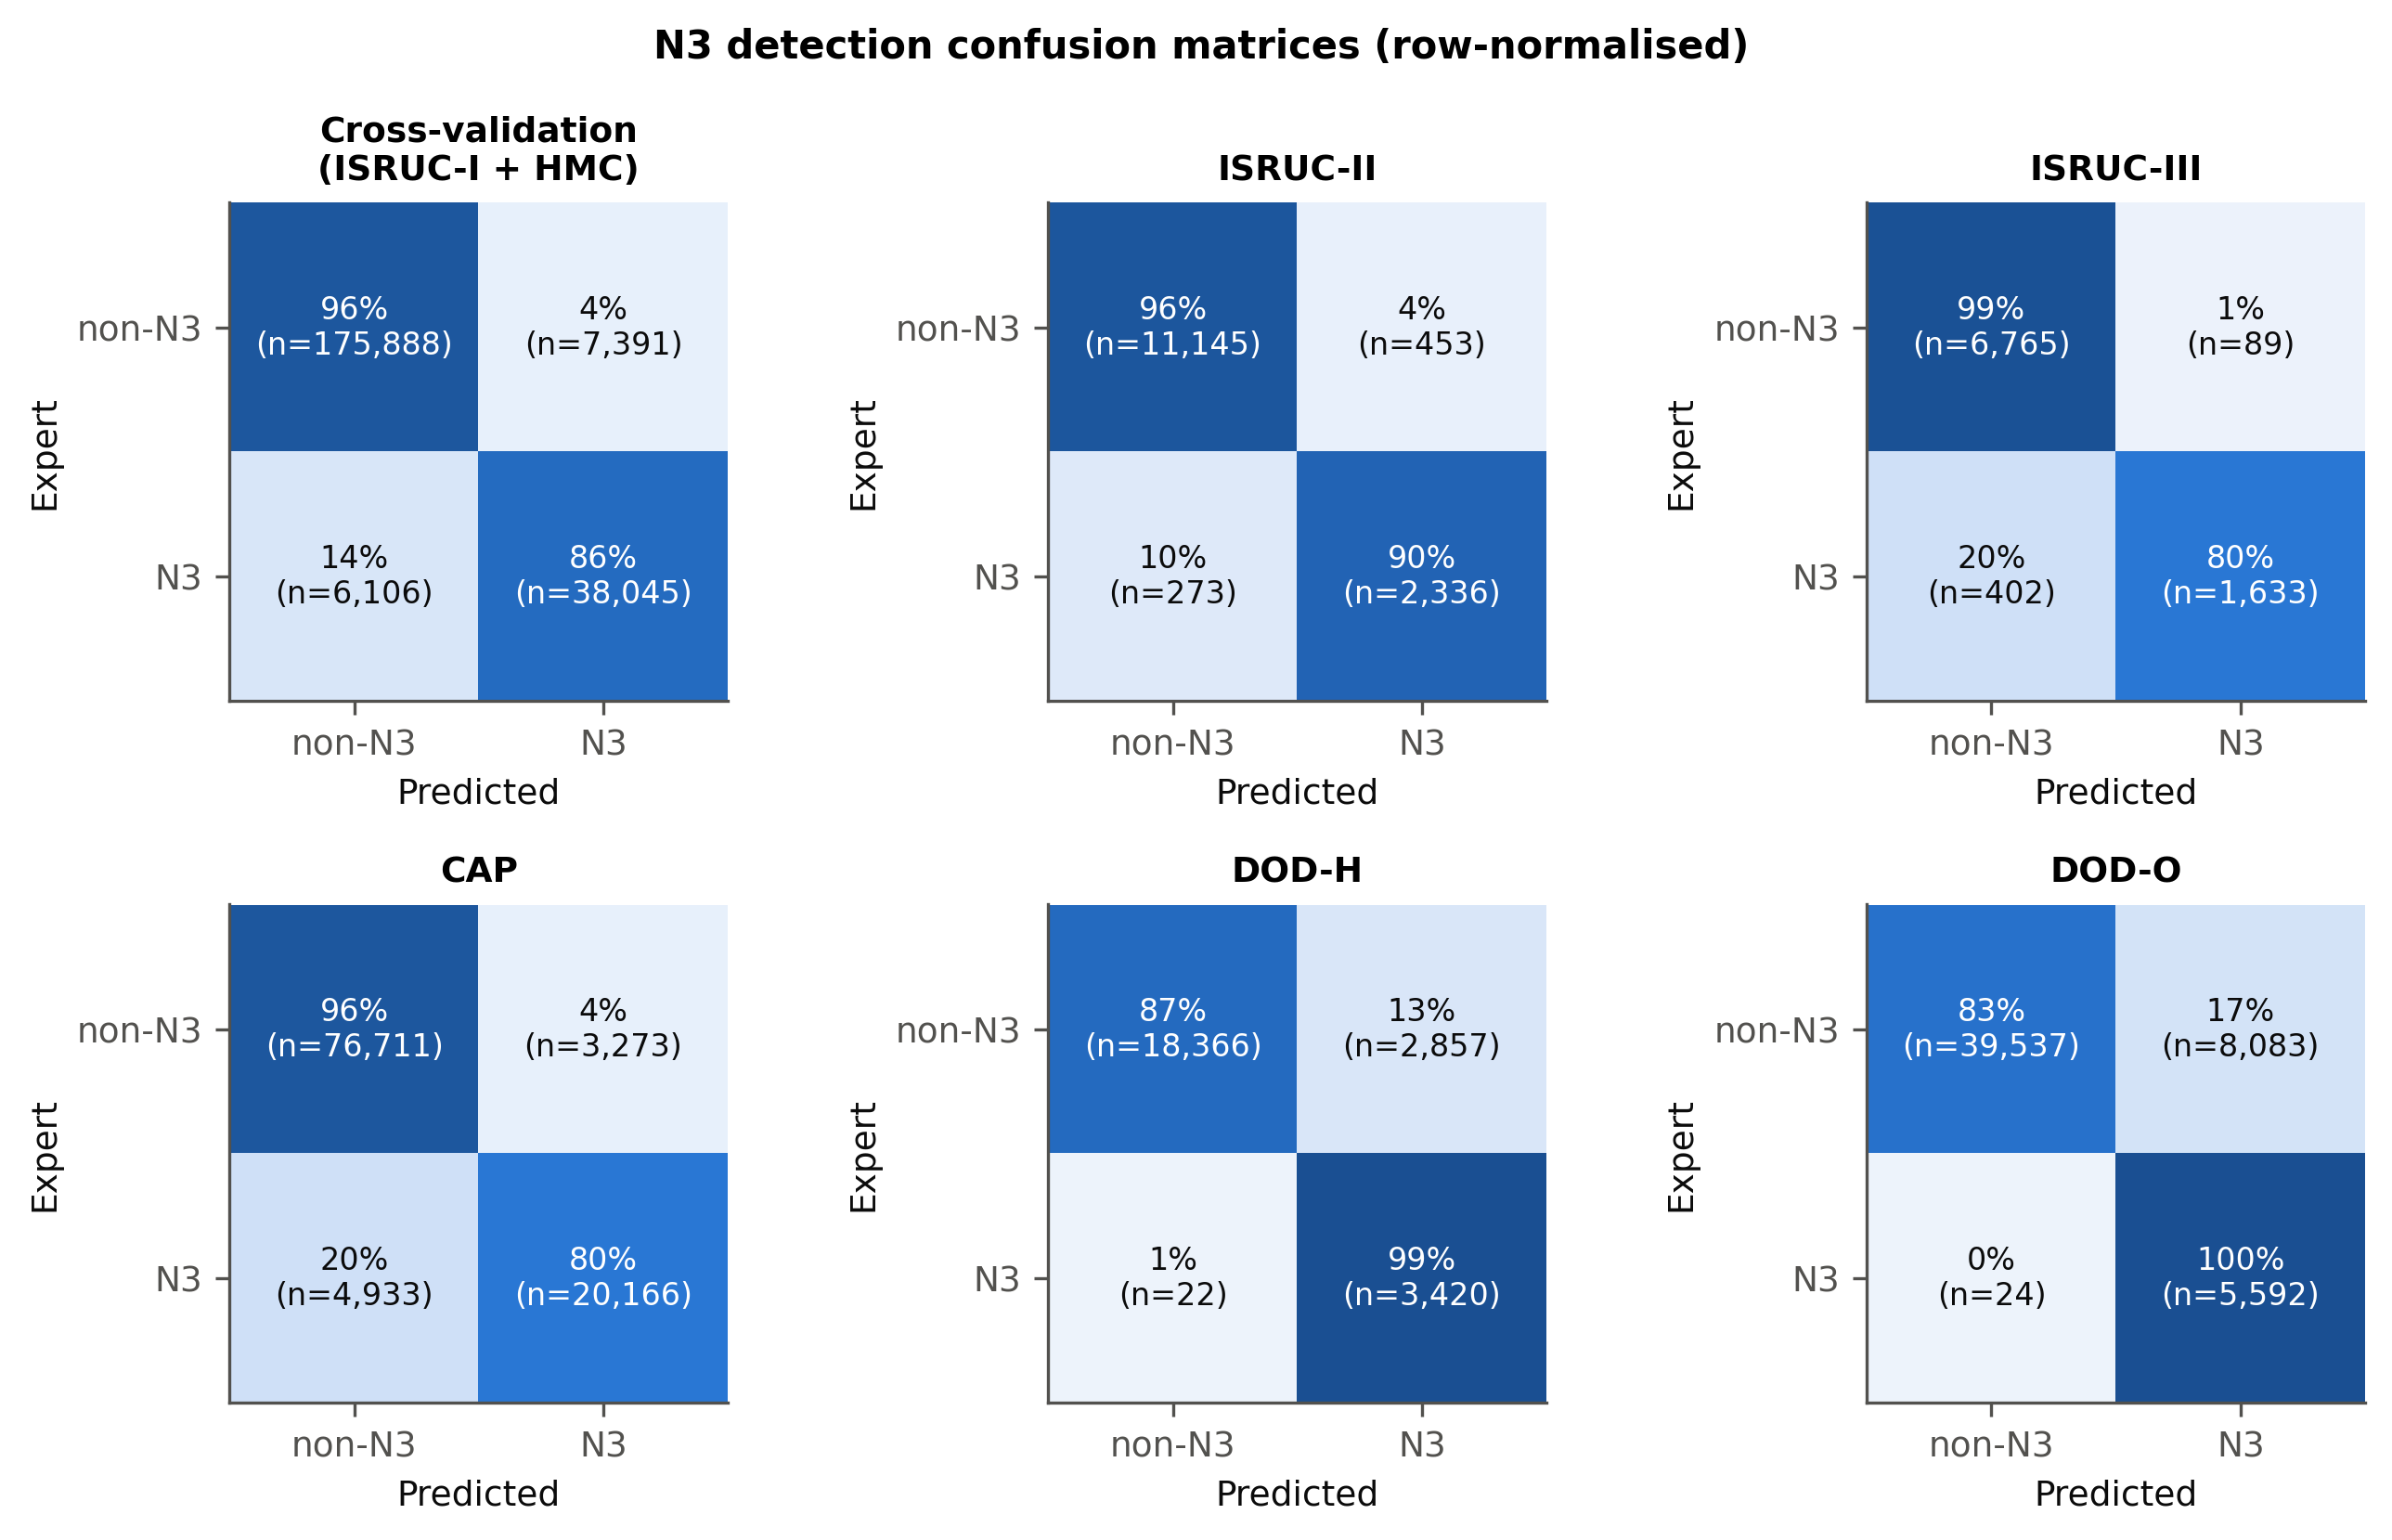
\includegraphics[width=0.5\columnwidth]{fig_rq1_confusion_matrices.png}
\caption{Row-normalised confusion matrices for N3 versus non-N3 epochs (counts in brackets). DOD cohorts show near-complete recall with more false positives; 96\% of these were scored N2 by the consensus.}
\label{fig:cm}
\end{figure}

% fig caption 96%: sensitivity_rq1_false_positive_structure.csv fp_expert_N2 DOD-H 0.966, DOD-O 0.964

The false positives in DOD did not occur at random. Of the DOD-O false positives, 96.4\% were consensus N2 epochs and 60.9\% had at least one of the five experts voting N3; in DOD-H the figures were 96.6\% and 51.0\%. In a post hoc analysis with a lenient reference (N3 if any expert scored N3), F1 rose to 0.834 in DOD-H and 0.819 in DOD-O; on epochs on which all experts agreed it was 0.740 and 0.550. Leave-one-cohort-out models reached DOD F1 scores between 0.624 and 0.739, so the drop is not caused by the ensemble. After temperature scaling, the expected calibration error was 0.022--0.061 in cross-validation, ISRUC and CAP, but 0.192 (DOD-H) and 0.225 (DOD-O) (Fig.~S2). % sensitivity_rq1_false_positive_structure; sensitivity_matrix; rq1_detection_metrics LOCO rows; ledger_extra ECE

\textit{Comparison with human scorers.} In ISRUC-I and ISRUC-II, the model agreed with single experts more closely than the experts agreed with each other (mean F1 0.867 vs 0.849 and 0.883 vs 0.861); this was true for each scorer separately (lowest model--scorer F1 0.858 and 0.866), although in ISRUC-I the model was trained, out of fold, on labels of the first scorer from the same centre. In DOD-O, where experts agreed least (mean pairwise F1 0.603, range 0.494--0.701), model--expert agreement (0.588, range 0.485--0.762) was inside the expert range. In DOD-H (0.695 vs 0.772, expert range 0.708--0.806) and ISRUC-III (0.881 vs 0.917), it was lower. % rq1_interrater_benchmark.csv


\subsection{Same-protocol comparison}
Table~\ref{tab:sota} shows the four published architectures trained under the same protocol. The proposed detector and DeepSleepNet did not differ significantly (median participant difference in F1 +0.005, Holm $p$ = 0.15; Fig.~S3), although DeepSleepNet has 264 times more parameters and needed 36.2 instead of 1.6 minutes per fold (wall-clock times on shared cloud GPUs, indicative only). The detector outperformed TinySleepNet (+0.011, $p$ = 0.0032), L-SeqSleepNet (+0.021, $p = 1.6\times10^{-8}$) and AttnSleep (+0.031, $p = 9.5\times10^{-18}$). Among the five same-protocol models, it had the highest external F1 score in ISRUC-II, DOD-H and DOD-O (0.866, 0.704, 0.580); DeepSleepNet was highest in CAP (0.836 against 0.831), and TinySleepNet and L-SeqSleepNet in ISRUC-III (0.903 against 0.869); all external values are in the repository. The pretrained open stager YASA, applied without any change, reached F1 scores of 0.79 in the training cohorts, 0.60--0.77 in ISRUC-II, ISRUC-III and CAP, and 0.79 and 0.72 in DOD-H and DOD-O; like the proposed detector, its precision dropped in DOD (0.66 and 0.57, compared with 0.87--1.00 elsewhere) while recall rose to 0.97. Its five-class decision is more cautious than our F1-optimised threshold, so the precision--recall area gives a fairer comparison: 0.907, 0.893, 0.910, 0.885, 0.962 and 0.864 in the training cohorts, CAP, DOD-H, DOD-O, ISRUC-III and ISRUC-II, compared with 0.933, 0.919, 0.946, 0.883, 0.968 and 0.905 for the proposed detector, on the same epochs in every cohort. % posthoc3_isruc2_same_nights.csv % posthoc2_yasa_comparator.csv % rq1_sota_comparison.csv, rq1_sota_paired_tests.csv

\begin{table}[!t]
\caption{Same-protocol comparison: cross-validation F1 (95\% CI), PR area, parameters and training time per fold. $\Delta$F1: median paired participant difference (proposed minus baseline) with Holm-corrected $p$.}
\label{tab:sota}
\centering
\setlength{\tabcolsep}{2pt}
\footnotesize
\begin{tabular}{@{}lccrrr@{}}
\toprule
Model & CV F1 & PR area & Params & min & $\Delta$F1 ($p$) \\
\midrule
Proposed & 0.849 (0.838--0.861) & 0.933 & 96k & 1.6 & -- \\ % rq1_sota_comparison
DeepSleepNet & 0.846 (0.835--0.857) & 0.925 & 25.4M & 36.2 & +0.005 (0.15) \\
TinySleepNet & 0.841 (0.829--0.852) & 0.925 & 1.5M & 4.5 & +0.011 (0.0032) \\
AttnSleep & 0.817 (0.803--0.829) & 0.904 & 513k & 36.1 & +0.031 ($<$0.001) \\
L-SeqSleepNet & 0.826 (0.812--0.839) & 0.907 & 208k & 4.7 & +0.021 ($<$0.001) \\
\bottomrule
\end{tabular}
\end{table}

\subsection{Validity of the factor scores}
In detected N3 of the training cohorts, delta intensity was 8.8 points higher in the first than in the second half of the night (95\% CI 6.8--10.8, $n$ = 213 participants), slow-wave morphology 9.0 (7.0--11.4), spectral dominance 4.5 (2.8--7.5) and the rating 7.2 (5.4--8.9); all $p < 10^{-5}$ (Fig.~S4). Continuity was also higher early in the night ($p = 3.3\times10^{-6}$), but its median difference was zero because most N3 epochs have only N3 neighbours. Expert N3 epochs scored higher than expert N2 epochs on every factor (median differences 30.8--37.8 points for the three signal factors, 249 participants; Fig.~S5). For delta intensity, morphology and the rating, the decline was repeated in all five external cohorts, and in CAP it was found for every factor. % rq2_factor_validity.csv

The scores also followed the graded judgement of human experts (Fig.~\ref{fig:graded}). On epochs that every expert scored as N2 or N3, each score increased with the fraction of experts who chose N3. The median within-participant Spearman correlation across 198 participants was 0.74 for delta intensity, 0.76 for morphology, 0.75 for spectral dominance and 0.81 for the rating, and it ranged from 0.79 to 0.81 for the rating in every cohort. Without the detector-derived continuity factor, the signal-only composite reached 0.76. When only detected N3 epochs were used, which tests the within-N3 claim directly, the correlations were lower but still positive in every cohort (rating median 0.56, from 0.26 in ISRUC-III to 0.80 in DOD-H; composite 0.53); in ISRUC, with two scorers, the expert fraction has only three levels. The signal factors are calculated from the EEG alone (expert labels are used only for the percentile scale of the training fold, a monotone transform that does not change a Spearman correlation). This agreement therefore shows convergent validity with the visual feature that experts score, not an independent physiological reference. Morphology and the grade use the same amplitude-and-coverage definition that experts apply, so part of this agreement follows from the definition. % rq2_factor_validity.csv graded rows

\begin{figure*}[!t]
\centering
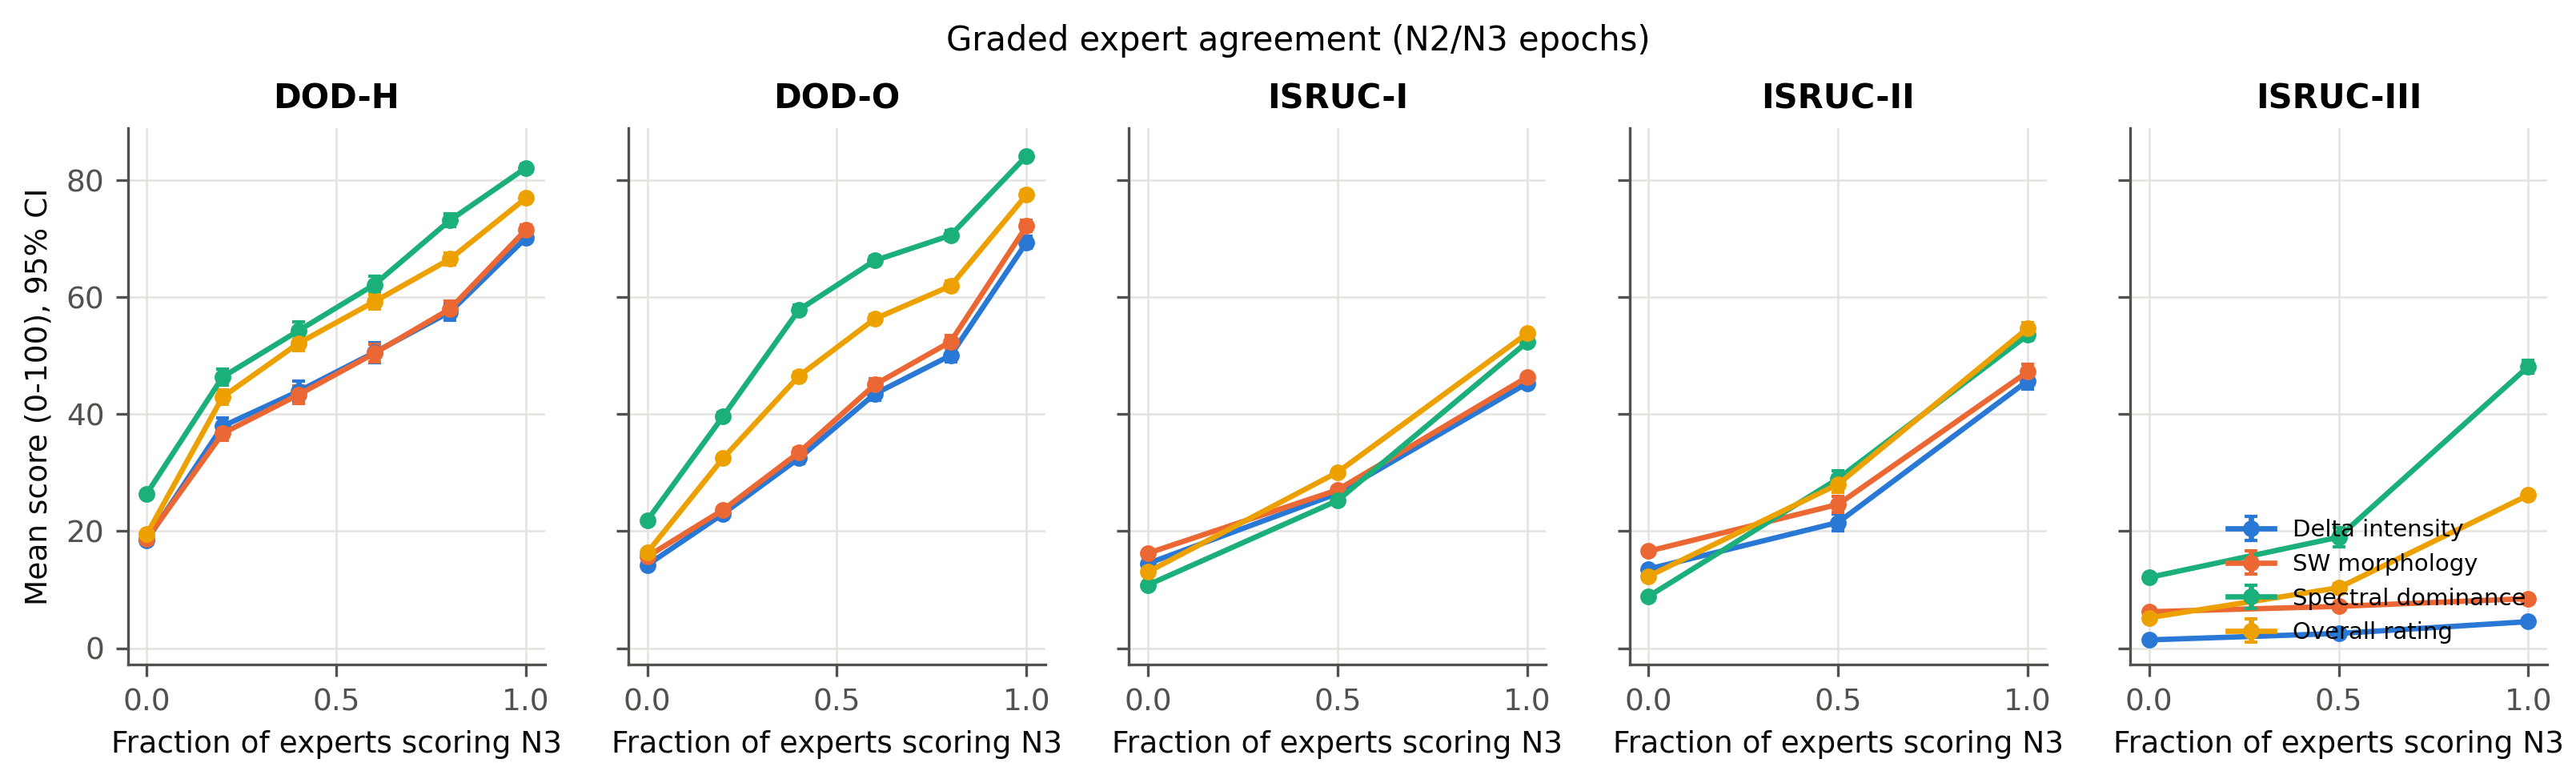
\includegraphics[width=0.56\textwidth]{fig_rq2_graded_expert_agreement.png}
\caption{Graded expert agreement. Mean factor scores and rating (95\% CI) by the fraction of experts who scored an epoch as N3, restricted to epochs scored N2 or N3 by every expert. DOD: five experts; ISRUC: two experts. The low absolute level of the amplitude-dependent scores in ISRUC-III is discussed in Section~\ref{sec:limitations}.}
\label{fig:graded}
\end{figure*}

\subsection{Within-N3 slow-wave grade}
In CAP, slow-wave coverage separated expert stage 4 from stage 3 epochs with an area of 0.782 over all stage 3/4 epochs and 0.743 over epochs that the detector also labelled N3. The prespecified criterion (0.75 on detected epochs) was therefore missed by 0.007. Within participants, the median area was 0.811. The grade was cautious: 98.7\% of stage 3 epochs were not graded High, but only 21.1\% of stage 4 epochs were graded High (Cohen's $\kappa$ 0.15; grade shares in Table~SIII). The High share was larger early in the night ($p = 1.9\times10^{-22}$), the grade rose with the expert vote (epoch-level $\rho$ = 0.318), and the High share was stable across the two ISRUC-II nights (ICC 0.988, $n$ = 8). The thresholds come from both scoring systems and the validation reference is scored with Rechtschaffen and Kales rules, so this shows agreement with R\&K stage 3/4 rather than with AASM N3 grading. % rq2_rk_grade_validation.csv, rq2_n3_grade_validity.csv, sensitivity_rq2b.csv


\subsection{Stability of the rating}
Under random Dirichlet perturbation of the weights around the prior, the 5th-percentile Spearman correlation with the prior-weighted rating was 0.979. Equal weights and weights from the first principal component gave correlations of 0.989 and 0.998, and dropping any single factor kept the correlation between 0.977 and 0.992. In the eight ISRUC-II participants recorded twice, the median nightly rating had a test--retest ICC of 0.763 (95\% CI 0.23--0.95), compared with 0.658 (0.01--0.92) for predicted N3 minutes and $-$0.008 ($-$0.63 to 0.65) for expert-scored N3 minutes. Delta intensity and morphology were similar (Fig.~S6, Table~SIV); spectral dominance was not stable (0.339). With only eight participants the intervals overlap, so this comparison is descriptive. % rq3_overall_rating_stability.json, rq7_profile_agreement.csv test-retest rows

\subsection{Component contributions}
The temporal-context block gave the largest gain (F1 +0.023, 95\% CI 0.018--0.027, Holm $p = 7.3\times10^{-16}$), and the convolutional backbone outperformed a features-only gradient-boosting model by 0.036 (Table~SII). Without the context block, none of the other components changed F1 significantly. Three training seeds of the full model gave F1 scores of 0.849, 0.844 and 0.844 (standard deviation 0.003), so differences below about 0.005 should not be interpreted. In the post hoc leave-one-component-out analysis from the full model, removing feature fusion lowered F1 by 0.0071 (95\% CI 0.0030--0.0108, Holm $p$ = 0.018), an effect larger than the largest seed-to-seed difference (0.0042; Fig.~S7). Removing class weighting or attention, shortening the context to $\pm$3 epochs, or restricting the features to the ten delta-related ones did not change F1 more than seed variability. % rq4_component_effects.csv, rq4_seed_variability.csv, rq4_extended_component_effects.csv



\subsection{Explanations}
Removing the delta band reduced the N3 probability by a median of 0.456, against 0.0005 for the alpha band, and delta was the top band for both perturbation and integrated gradients in all 600 epochs (one to five per participant). The rank correlation between the two methods across bands was 0.7, and the Shapley surrogate (fidelity $R^2$ = 0.86) also ranked the delta feature group first. The same delta dominance held for false positives, false negatives and external cohorts (Fig.~S8). Because N3 is defined by delta waves and delta features are among the inputs, this dominance is expected and is a consistency check rather than evidence that the network learned slow waves. Attention weights correlated weakly and negatively with slow-wave locations (median $\rho = -0.13$), so we do not use attention as an explanation. % rq5_summary.json, rq5x_band_importance_by_outcome.csv

\subsection{Reliability}
The cross-fitted reliability score found misclassified epochs with an area of 0.879 (Fig.~S9). Excluding the 20\% least reliable epochs raised F1 from 0.849 on all epochs to 0.949 on the remaining 80\%, while keeping 72\% of expert N3 and 64\% of expert N2 epochs, and the error rate was 0.9\% in the high, 13.1\% in the medium and 24.6\% in the low category. Most of the signal came from model confidence (0.872) and the Mahalanobis distance (0.855; Table~SV); the quality-control flags alone did not detect errors (areas 0.30--0.48). The score also identified epochs on which the two ISRUC-I experts disagreed (area 0.883). Externally, the area was 0.853 in CAP, 0.872 in ISRUC-II and 0.941 in ISRUC-III but 0.751 in DOD-H and 0.689 in DOD-O, where confidence alone reached 0.683 and 0.612. % rq6_reliability_components.csv, rq6_reliability_categories.csv, rq6_risk_coverage.csv, sensitivity_rq6.csv


\subsection{Episodes and overnight profile}
\begin{figure}[!t]
\centering
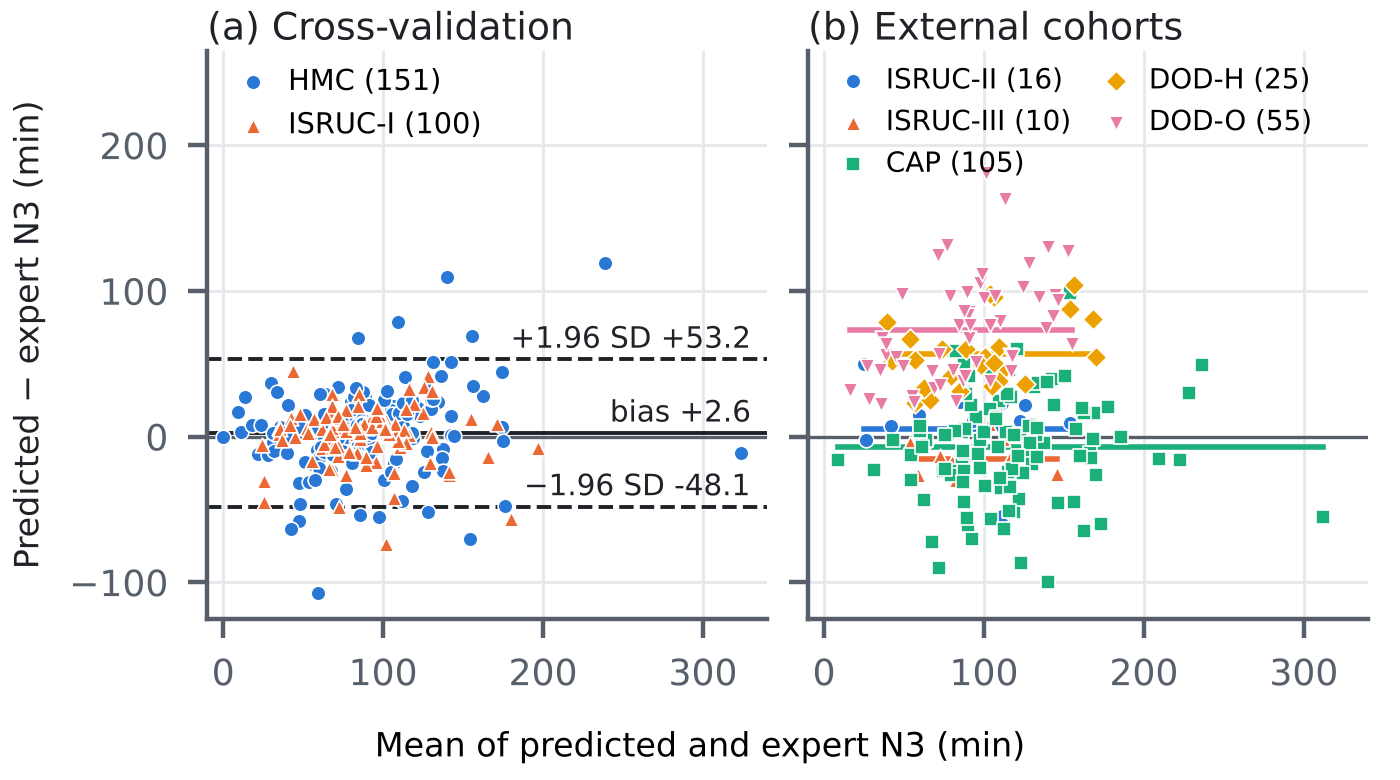
\includegraphics[width=0.86\columnwidth]{fig_rq7_bland_altman_main.png}
\caption{Bland--Altman plots of nightly N3 minutes, predicted minus expert. (a) Cross-validation with bias and 95\% limits of agreement. (b) External cohorts; horizontal lines show each cohort's mean difference. Numbers in brackets are recordings (ISRUC-II: two nights of eight participants).}
\label{fig:ba}
\end{figure}

Predicted and expert N3 minutes per night agreed with ICC 0.806 (95\% CI 0.758--0.845) in cross-validation (bias +2.6 min, limits $-$48.1 to 53.2 min; Fig.~\ref{fig:ba}a). The share of N3 in the first half of the night (0.929), the longest episode (0.780) and the median rating (0.950) also agreed; the episode count (0.622) and median episode duration (0.431) agreed less and are treated as exploratory. Externally, N3 minutes agreed in ISRUC-II (0.898 and 0.740 for the first and second night, eight participants each), ISRUC-III (0.794) and CAP (0.730), but not in DOD-H (0.403) or DOD-O (0.222), where the detector added on average 56.7 and 73.3 min of N3 per night (Fig.~\ref{fig:ba}b). The consistency ICC(3,1) in DOD-H (0.826) and DOD-O (0.590) shows that the order of nights was mostly kept and that most of the disagreement is a constant offset, the same boundary shift that we saw at the epoch level. Fig.~S10 shows one example night. % rq7_profile_agreement.csv



\subsection{Added value over the detector output (post hoc)}
These analyses were added after the first full run and are exploratory: they were not among the prespecified criteria, and their p-values are corrected within each comparison, not across the section. To test whether the description adds information to the detector itself, we evaluated the N3 logit, the calibrated N3 probability (a monotonic transform with the same results) and a signal-only composite with the same references. The expert-based references favoured the logit, which was trained on expert labels: its graded-vote correlation was 0.839, against 0.807 for the rating and 0.764 for the composite, and its CAP stage 4/3 area was 0.860, against 0.776 and 0.764. On the night-time decline, which does not depend on expert scoring, morphology and delta intensity were higher early than late on detected epochs in 83.6\% and 80.8\% of cross-validated and 84.7\% and 83.2\% of external participants, against 73.2\% and 75.3\% for the logit. Because detected epochs are selected by the logit, the primary test is the paired comparison of per-participant early--late areas, which showed that slow-wave morphology declined more strongly than the logit, both on detected N3 epochs (median area 0.673 against 0.635 in cross-validation) and on expert N3 epochs, which are not selected by the logit (0.697 against 0.664; externally 0.712 against 0.660; Holm $p < 0.001$). Delta intensity also declined more strongly on detected epochs (Holm $p \le 0.012$) and on external expert N3 epochs ($p = 0.008$) but not on cross-validated expert N3 epochs ($p = 0.054$); spectral dominance declined less, and the rating and composite did not differ from the logit. When expert N2 epochs were included, the logit was equal to or better than all factors except slow-wave morphology. In CAP, where age and sex are available (102 participants aged 14--82 years, each with at least ten expert N3 epochs, median 235 epochs per participant), every factor score decreased with age (Spearman $\rho$ from $-0.48$ to $-0.70$, $p < 10^{-6}$), also after adjustment for diagnosis (partial $\rho$ from $-0.28$ to $-0.38$, $p \le 0.006$) and within the 13 healthy controls ($\rho$ from $-0.59$ to $-0.81$), but not within the REM sleep behaviour disorder group, which has a narrow age range (58--82 years). The amplitude-dependent scores were higher in women ($p \le 0.014$). % posthoc_within_n3_comparators.csv; posthoc2_paired_decline.csv; posthoc2_age_association.csv

\subsection{Sensitivity analyses}
Of 194 post hoc sensitivity settings, 180 tested a conclusion, and the conclusion held in 129 (Table~SVI). Most of the 51 exceptions concern the continuity factor, whose median early--late difference is zero by construction (13), the longest-episode agreement (14) and the DOD cohorts (13), consistent with Section~\ref{sec:dod}; the rest are four single external contrasts, two N3-minute agreements (CAP 0.728), four leave-one-component-out contrasts within seed variability and one extreme weight perturbation (rating correlation 0.81). For this reason, episode-level outputs are exploratory. % sensitivity_matrix.csv

\section{Discussion}
This study shows that one central EEG channel can detect deep sleep and describe it in physiological terms. Four findings stand out. First, a compact detector matched DeepSleepNet, which has 264 times more parameters, and outperformed three other re-implemented architectures under the same protocol, mainly thanks to temporal context \cite{phan2022sleeptransformer,phan2023lseqsleepnet}. Second, it ranked N3 epochs almost as well in five independent cohorts as in cross-validation, and where experts agreed least, its agreement with them was within their own range. Third, the transparent scores followed known slow-wave physiology: they decreased across the night \cite{borbely2016twoprocess,riedner2007slowwaves} and with age, and rose with the share of experts who scored N3. Fourth, the reliability score identified the epochs that need review. % rq1_sota_paired_tests, rq4_component_effects, rq1_interrater_benchmark

\subsection{Implications for long-term monitoring of deep sleep}
Large studies of slow-wave sleep and brain health \cite{xie2013clearance,baril2021brainaging,himali2023dementia} need measures that are cheap, repeatable and understandable. Single-channel home EEG can match polysomnography for slow-wave activity \cite{lucey2016singlechannel}, but wearables rarely measure slow-wave sleep accurately \cite{green2022devices}. Our method needs one central channel and 96,226 parameters, reports only physiologically named numbers with an exact additive breakdown, and gives every epoch a reliability score. Excluding the least reliable fifth raised F1 on the remaining epochs to 0.949, but reliability was weaker in DOD (area 0.751 and 0.689), where the detector is least accurate, so any monitoring use would need a check of this kind before its output is trusted. % rq6_risk_coverage

\subsection{Interpreting the Dreem results}
\label{sec:dod}
The DOD results are the main limitation of the detector. The evidence suggests that the problem is where the reference places the N2/N3 boundary, not a failure to see slow waves. The ranking of epochs and the order of nights transferred to DOD (Fig.~\ref{fig:ba}b). False positives were mostly consensus N2 epochs with less automatically detected slow-wave coverage than true positives (median 4.6\% against 18.5\% in DOD-O). This fits DOD scorers placing the boundary higher, although automated coverage is generally lower than visual coverage. The same pattern appeared without class weighting (DOD-O precision 0.415), and YASA showed the same precision drop in DOD; its more cautious operating point gave a higher DOD F1 but a lower F1 elsewhere. A threshold chosen for each cohort on test labels would raise the DOD F1 score, but it would make the external evaluation invalid. % rq1_detection_metrics; sensitivity_rq1_false_positive_structure; rq4_variant_external_metrics; rq7_profile_agreement icc31

Calibration showed a related effect (Section~IV-A). Positive-class weighting can move the logits by a constant amount that a single temperature cannot remove \cite{guo2017calibration}. Without class weighting, the cross-validated error fell from 0.060 to 0.006, and Platt scaling of the primary model reached 0.003; in DOD both corrections reduced it to 0.11--0.15, and in the other external cohorts it stayed at or below 0.044. This is consistent with the logit-shift explanation, the remaining DOD error fits the boundary shift, and Platt scaling is a simple correction in practice. % posthoc_calibration.csv

\subsection{What the factor scores measure}
The factor scores describe slow-wave strength in one EEG derivation and are meant as research measures. They are not validated measures of clinical, subjective or restorative sleep quality, because none of our datasets contains such a reference. Their agreement with the graded expert vote is convergent validity: the scores measure, on a continuous scale, the slow activity that makes experts vote N3, and so turn expert disagreement into a graded quantity. Because morphology uses the amplitude-and-coverage definition that experts apply, part of this agreement follows from the definition, so it is a consistency check rather than independent validation. The approach is in line with the hypnodensity view of stage ambiguity \cite{bakker2023ambiguity,huijben2023hypnodensity} and with concerns about fixed N3 criteria \cite{davidson2025n3}. The exploratory post hoc comparison suggests that the two outputs play complementary roles. The detector logit, trained on expert labels, matched expert judgement best and is the better number for ranking epochs as experts would. Slow-wave morphology followed the homeostatic decline, which does not depend on expert scoring, more strongly than the logit, also on epochs not selected by the detector, and delta intensity did so in most comparisons. The scores also decreased with age, as slow-wave amplitude and other EEG features do \cite{rosinvil2021age,mai2025aisleep}, even after adjustment for diagnosis, and, unlike the logit, they are named, additive and comparable between nights. The combined rating matched the logit on the decline. The test--retest data from eight participants are consistent with stability but too small to confirm it. % rq2_factor_validity graded; posthoc_icc_ci

Because the factors are strongly correlated, the rating hardly depends on the prior weights, and its exact additive breakdown shows which factor caused a given value. % rq3_overall_rating_stability.json

\subsection{The slow-wave grade}
The grade came close to its criterion (0.743 against 0.75) and was cautious: almost no stage 3 epoch was graded High, but only one in five stage 4 epochs was. A likely reason is that automated coverage from a filtered channel is lower than a scorer's visual estimate. The thresholds come from both scoring systems and the reference is R\&K-scored CAP, so this result does not establish agreement with AASM grading. A lower High threshold would have to be learned from the test reference, so we report the grade as not yet validated; the continuous rating (0.776) and the detector logit (0.860) separated stage 4 from stage 3 better. % rq2_rk_grade_validation; sensitivity_rq2b

\subsection{Reliability and explanations}
The reliability score separates likely errors well in the training cohorts, ISRUC and CAP, and it identifies epochs on which human experts disagree. This matches what ensemble and Monte Carlo uncertainty achieve for five-class staging \cite{dei2025sleepyland,vainikka2026uncertainty}. The quality-control flags did not predict errors because the detector makes its mistakes on clean N2/N3 boundary epochs, not on artefacts. In DOD, error detection was weaker, as expected for a systematic boundary shift, although the out-of-distribution and quality components helped most there. Both explanation methods ranked the delta band first in all analysed epochs, including errors. Because N3 is defined by delta waves, this is consistent with the physiology that defines N3, but it does not by itself show that the network learned slow waves. % rq6_reliability_components; sensitivity_rq6; rq5x

\subsection{Limitations}
\label{sec:limitations}
First, public data contain no expert ratings of slow-wave strength, so the factor scores and grade are research descriptors tested only against indirect references; a blinded annotation of within-N3 slow-wave strength by several raters is the natural next step, and the open code makes such a study straightforward. Second, in ISRUC-III the amplitude-dependent factors were close to the floor even for expert N3 epochs (median delta-intensity percentile 4.6 against 44.2 in ISRUC-I), while the scale-free spectral factor was normal (47.1). This points to an amplitude-scale difference in the source files of this cohort; the amplitude-dependent YASA also found only 43\% of expert N3 epochs there. Detection, which uses recording-normalised input, and the within-participant analyses are not affected, but absolute scores and grades in ISRUC-III cannot be interpreted. Third, individual age and sex are available only for CAP. There, the age association held after adjustment for diagnosis, but because the scores depend on age and sex \cite{davidson2025n3,rosinvil2021age}, absolute values can only be compared within a similar population and recording set-up, and age-specific references are needed. Fourth, all cohorts used a central-mastoid derivation; frontal and wearable montages need their own percentile references and evaluation. Fifth, the test--retest analysis is based on only eight participants. Sixth, the baselines were re-implemented with a shared recipe (Table~SI) and may perform below their best published configurations. Seventh, the DOD labels needed an alignment step that uses labels, and a label-free alignment has not yet been tested. Eighth, DOD-O is an obstructive sleep apnoea population whose arousals and architecture differ from the training cohorts. Finally, the post hoc analyses do not affect any verdict; Table~SVI lists where their conclusions differed. % ledger_extra 4.6, 44.2, 47.1

\section{Conclusion}
One central EEG channel was enough to detect N3 sleep in seven cohorts. Ranking performance (ROC area at least 0.96) was high in every cohort, F1 was lower in the two Dreem cohorts, and accuracy matched DeepSleepNet and exceeded three other published architectures trained under the same protocol, with only a fraction of their parameters. When the detector disagreed with external references, it mostly did so on epochs on which the experts themselves were divided: 51--61\% of the Dreem false positives had at least one expert voting N3. For every detected epoch, transparent factor scores and an additive rating described slow-wave strength, decreased across the night and followed the fraction of experts who scored the epoch as N3, and a reliability score showed which epochs need review. In exploratory post hoc analyses, slow-wave morphology followed the night-time decline more closely than the detector output, and in CAP the scores decreased with age. The three-level grade came close to, but did not reach, its prespecified agreement with expert stage 3/4 scoring. Together, these results show that deep sleep can be detected with high ranking accuracy, described transparently and checked for reliability from a single channel, giving an open and reproducible basis for long-term studies of slow-wave sleep and brain health. The next steps are expert annotation of slow-wave strength within N3 and evaluation on wearable montages. % sensitivity_rq1_false_positive_structure 0.510, 0.609


\section*{Data and code availability}
All recordings are public: ISRUC-Sleep \cite{khalighi2016isruc}, the Haaglanden Medisch Centrum database \cite{alvarez2022hmcdb,alvarez2021hmc} and the CAP Sleep Database \cite{terzano2001cap} on PhysioNet \cite{goldberger2000physionet}, and the Dreem Open Datasets \cite{guillot2020dod}. No data are redistributed. The code, the executed notebooks and every result table and figure of the reported run are available at \url{https://github.com/alampranto17/SPF-SleepNet-Research} (folder \texttt{v2}, run \texttt{20261030-1528}).

\section*{Ethics statement}
This study used only publicly available, de-identified recordings released for research by the original investigators \cite{khalighi2016isruc,alvarez2021hmc,guillot2020dod,terzano2001cap}. No new data were collected. \placeholder{AUTHOR INPUT: confirm with your institution whether an exemption statement or reference number is required.}

\section*{Acknowledgment}
An AI system (Claude, Anthropic) assisted in drafting the text of all sections, the analysis code and the figures. The authors designed the study, checked every analysis, number and reference against the code outputs, and take full responsibility for the content. \placeholder{AUTHOR INPUT: confirm this disclosure; add other acknowledgments.}

\bibliographystyle{IEEEtran}
\bibliography{refs}

\end{document}
